\chapter{モータ特性表自動生成ツール}\label{cha:Tool}
本章では、 本研究で試作するモータ特性表自動生成ツールについて説明する。
モータ特性表自動生成ツールは、モータのシミュレーション結果から、\ref{mortoku}節で述べたモータ特性表を自動生成する。
モータ特性表自動生成ツールの処理の流れを、図\ref{fig:kouzou}に示す。
\begin{figure}[t]
	\centering
	% \includegraphics[width=16.5cm]{./Image/.png}
	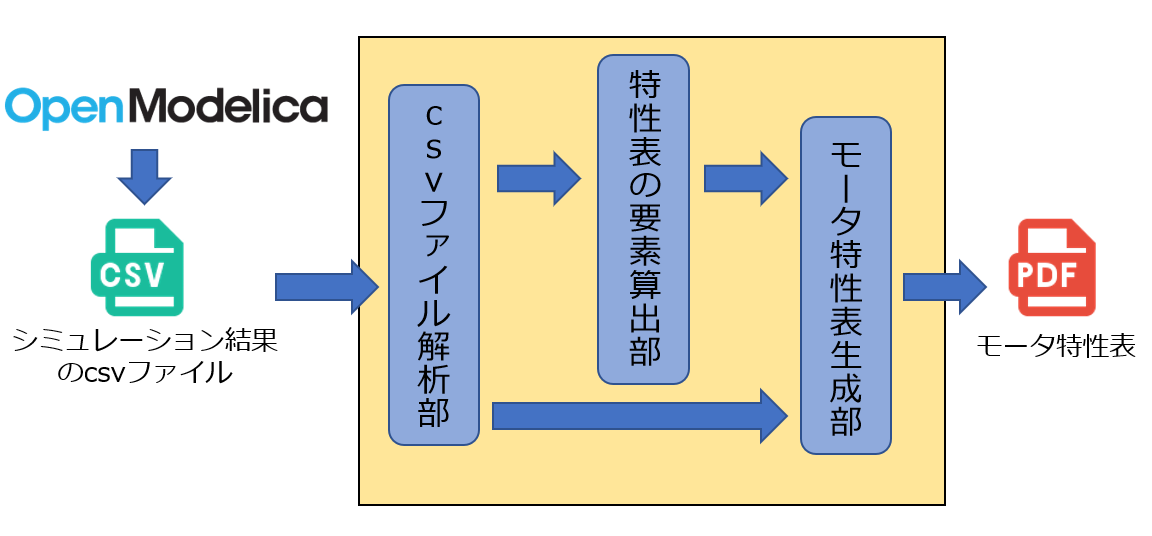
\includegraphics[width=14cm]{./Image/kouzou.png}
    \caption{モータ特性表自動生成ツールの構造}
	\label{fig:kouzou}
  \end{figure}
モータ特性表自動生成ツールの入力は、モータに関してシミュレーションしたOpenModelicaから出力されるcsvファイルである。ここで、現時点のツールは、入力となるcsvファイルは
次の3つの制約をすべて満たす必要がある。
\begin{itemize}
    \item \ref{taioumodel}節で述べた2つのモデルを対象とする
    \item モータの回路に印加する電圧値は一定とする
    \item 0秒からモータに入力を与える
\end{itemize}


モータ特性表自動生成ツールは、3つの処理部で構成しており、それぞれ以下の処理を行う。
\begin{itemize}
    \item csvファイル解析部
    \begin{itemize}
        \item 実行コマンドの取得
        \item csvファイルの読み込み
    \end{itemize}
    \item 特性表の要素算出部
    \begin{itemize}
        \item 基礎データの算出
        \item 特性表の構成要素の算出
    \end{itemize}
    \item モータ特性表生成部
    \begin{itemize}
        \item 特性表の生成
        \item 特性グラフの生成
        \item モータ特性表の生成
    \end{itemize}
\end{itemize}
以下に、それぞれの処理部について説明する。
\section{csvファイル解析部}\label{csv_sec}
csvファイル解析部では、モータ特性表自動生成ツールを実行する際の実行コマンドから、読み込むcsvファイルを決定する。
そして、指定したcsvファイルを読み込み、モータ特性表を生成するために必要なデータを取得する。
以下に、各処理について説明する。
\subsection{モータ特性表自動生成ツールの実行}\label{sub:zikkou_tool}
読み込むcsvファイルを決定するために、モータ特性表自動生成ツールを実行するコマンドの引数に、csvファイル名を指定する。
モータ特性表自動生成ツールを実行するためのコマンドを、コード\ref{code:zikkou}に示す。
\begin{figure*}[t]
	\lstinputlisting[label={code:zikkou}, caption={実行コマンド}]{Image/comand.txt}
\end{figure*}
なお、この実行コマンドは、ツールの実行ファイルが存在するディレクトリで実行する必要がある。

第1引数には、入力とするcsvファイルのパスを含めたファイル名を指定する。

第2引数には、第1引数で指定したcsvファイルの中の、モータ特性表を自動生成したいモータのモデルに含まれる、慣性部品のオブジェクト名を指定する。

第3引数には、第1引数で指定したcsvファイルの中の、モータ特性表を自動生成したいモータのモデルに含まれる、電源部品のオブジェクト名を指定する。

第2引数と第3引数に、慣性部品と電源部品のオブジェクト名を指定する理由については、\ref{sub:csv_scan}節で述べる。

引数を取得するために、実行コマンドの引数を、1次元の配列で保持するsysライブラリのargvを使用する。
以下に、処理の流れを示す。

\begin{enumerate}
    \item argvの要素数を取得する
    \item argvの要素数が4以外であれば、図\ref{fig:error_hikisuu}のエラーを表示し、全体の処理を終了する
    \item argvの1番目の要素からcsvファイル名を取得する
    % \item 取得したファイル名の拡張子がcsvでない場合、図\ref{fig:error_file}のエラーを表示し、全体の処理を終了する
    \item argvの2番目の要素から慣性部品のオブジェクト名を取得する
    \item argvの3番目の要素から電源部品のオブジェクト名を取得する
    \item 取得したcsvファイル名、慣性部品のオブジェクト名、電源部品のオブジェクト名をもとに\ref{sub:csv_scan}節で述べる処理を実行する
\end{enumerate}

\subsection{csvファイルの読み込み}\label{sub:csv_scan}
モータ特性表の要素を算出するために必要なデータを、csvファイルから取得する。
今回、モータ特性表の自動生成に必要となるデータの導出計算式は、以下の通りである。
% \vspace{3zh}
\begin{itemize}
    \item 回転数
    \begin{eqnarray}
        \mbox{回転数 $(\mathrm{rpm})$} = \frac{60 \times \mbox{角速度 $(\mathrm{rad/s})$}}{2\pi}   \label{siki:speed}
    \end{eqnarray}

    \item 出力 
    \begin{eqnarray}
        \mbox{出力 $(\mathrm{W})$} = \mbox{ トルク $(\mathrm{N \cdot m})$} \times \mbox{角速度 $(\mathrm{rad/s})$} \label{siki:out}
    \end{eqnarray}
    \item 効率
    \begin{eqnarray}
        \mbox{効率 (\%)} = \frac{\mbox{出力 $(\mathrm{W})$}}{\mbox{入力 $(\mathrm{W})$}}  \times 100 \label{siki:effi}
    \end{eqnarray}
    \item 入力
    \begin{eqnarray}
        \mbox{入力 $(\mathrm{W})$} = \mbox{電圧値 $(\mathrm{V})$} \times \mbox{電流値 $(\mathrm{A})$}  \label{siki:in}
    \end{eqnarray}
    \item 定格出力
    \begin{eqnarray}
        \mbox{定格出力 $(\mathrm{W})$} = \mbox{最大効率時のトルク $(\mathrm{N \cdot m)}$} \times \mbox{最大効率時の角速度  $(\mathrm{rad/s})$} \times \frac{2\pi}{60} 
        \label{siki:teikaku}
    \end{eqnarray}
     
\end{itemize}

上記の式より、モータ特性表の要素を算出するために必要なデータは、トルク、角速度、電圧、電流である。
また、トルク、角速度、電圧、電流の値を持つcsvファイル内の変数名の拡張子を、表\ref{tab:hensuu}に示す。 
\begin{table}[t]
	\centering
	\caption{各データを持つ拡張子}
	\begin{tabular}{|c|c|} \hline
	  必要なデータ & 変数名 \\ \hline \hline
	  トルク値 & (慣性部品のモジュール名).flange\_a.tau \\ \hline
	  角速度値 &  (慣性部品のモジュール名).w \\ \hline
	  電圧値 &  (電源部品のモジュール名).p.v \\ \hline
	  電流値 &  (電源部品のモジュール名).n.i \\ \hline
	\end{tabular}
	\label{tab:hensuu}
  \end{table}

モータ特性表自動生成ツールで、csvファイルを読み込むために、表\ref{tab:libr}で挙げたcsvライブラリを使用する。csvライブラリを用いた場合、csvファイルを1行ごとに分けて読み込む。
以下に、csvファイルの読み込み処理の流れを示す。
\begin{enumerate}
    \item 取得したファイル名の拡張子がcsvでない場合、図\ref{fig:error_file}のエラーを表示し、全体の処理を終了する
    \item csvファイルを読み込み専用で開く
    \item csvファイルが開けなかった場合、図\ref{fig:error_file}のエラーを表示し、全体の処理を終了する
    \item csvファイルの各行に対して、以下の処理を繰り返す
    \begin{enumerate}
        \item csvファイルから取得した行の各列の値を保持する配列rowに格納する
        \item csvファイルの1行目を読み込んでいる場合、配列rowの要素数分、以下の処理を繰り返す
            \begin{enumerate}
                \item 変数名に、慣性部品のオブジェクト名が含まれている場合、以下の処理を行う
                \begin{enumerate}
                    \item 変数名の末尾に、「.flange\_a.tau」が含まれている場合、その変数名を格納している配列rowのインデックスを取得する
                    \item 変数名の末尾に、「.w」が含まれている場合、その変数名を格納している配列rowのインデックスを取得する
                \end{enumerate}
                \item 変数名に、電源部品のオブジェクト名が含まれている場合、以下の処理を行う
                \begin{enumerate}
                    \item 変数名の末尾に、「.p.v」が含まれている場合、その変数名を格納している配列rowのインデックスを取得する
                    \item 変数名の末尾に、「.n.i」が含まれている場合、その変数名を格納している配列rowのインデックスを取得する
                \end{enumerate}
            \end{enumerate}
            % \item 3.(a)で配列rowのインデックスを4つ取得するが、いずれか1つでも取得できない場合、図\ref{fig:error_comand}のエラーを表示し、全体の処理を終了する
            \item 4.(b)で配列rowのインデックスを4つ取得し、いずれか1つでも取得できない場合、図\ref{fig:error_comand}のエラーを表示し、全体の処理を終了する
  
        % \item csvファイルの2行目を読み込んでいる場合、以下の処理を行う
        % \begin{enumerate}
        %     \item トルク値の0.0秒段階の値を変数 torque\_defaultに代入する
        %     \item 角速度値の0.0秒段階の値を変数 angularvelocity\_defaultに代入する
        %     \item 電圧値の0.0秒段階の値を変数volyage\_defaultに代入する
        %     \item 電流値の0.0秒段階の値を変数 current\_defaultに代入する
        % \end{enumerate}
        \item csvファイルの2行目以下を読み込んでいる場合、以下の処理を行う
        \begin{enumerate}
            \item トルク値を格納する配列 torqueに、4.(b).i.A.で取得した配列rowのインデックスをキーに持つ値を格納する
            \item 角速度値を格納する配列 angularvelocityに、4.(b).i.B.で取得した配列rowのインデックスをキーに持つ値を格納する
            \item 電圧値を格納する配列 voltageに、4.(b).ii.A.で取得した配列rowのインデックスをキーに持つ値を格納する
            \item 電流値を格納する配列 currentに、4.(b).ii.B.で取得した配列rowのインデックスをキーに持つ値を格納する
        \end{enumerate}
    \end{enumerate}

\end{enumerate}
% なお、上記の処理の流れにおいて、
% csvファイルの2行目を読み込まない理由は、\ref{OM}節で述べたように、2行目にはモデルを作成した際の初期値が格納されており、初期値はモータ特性表の要素を算出することに使用しないからである。
\begin{figure}[t]
	\centering
	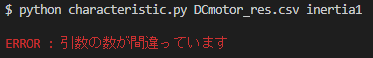
\includegraphics[width=10cm,height=1.5cm]{./Image/error_tarinai.png}
	\caption{引数の数に誤りがあった場合のエラー文の例}
	\label{fig:error_hikisuu}
\end{figure}
\begin{figure}[t]
	\centering
	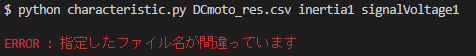
\includegraphics[width=12cm,height=1.5cm]{./Image/error_file.png}
	\caption{第1引数に誤りがあった場合のエラー文の例}
	\label{fig:error_file}
\end{figure}
\begin{figure}[t]
	\centering
	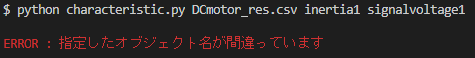
\includegraphics[width=12cm,height=1.5cm]{./Image/error_comand.png}
	\caption{第2引数、第3引数に誤りがあった場合のエラー文の例}
	\label{fig:error_comand}
\end{figure}

\section{特性表の要素算出部}\label{youso_sec}
特性表の要素算出部では、\ref{sub:csv_scan}節で取得したデータをもとに、特性表の各要素を算出する。
まず、特性表の各要素を算出するために必要となる基礎データを算出する。基礎データとは、回転数、出力、効率の値のことを指す。
そして、\ref{sub:csv_scan}節で取得したデータと、基礎データから特性表の各要素を算出する。
以下より、各処理について説明する。

\subsection{基礎データの算出}\label{sub:youso_kiso}
基礎データの算出処理では、回転数、出力、効率の値を持つ配列を、それぞれの値に対して生成する。
各配列の生成方法を以下に示す。以下の式で

\subsubsection{回転数}\label{sub:sub:kaiten}
% 回転数を算出する式は、\ref{sub:csv_scan}節の箇条書き中にある、回転数にて示した式を用いる。
回転数を算出する式は、%\ref{sub:csv_scan}節の
(\ref{siki:speed})式を用いる。
配列angularvelocityの各要素を、それぞれ(\ref{siki:speed})式に適用し、回転数の値を持つ配列speedを生成する。

\subsubsection{出力}\label{sub:sub:syutu}
% 出力を算出する式は、\ref{sub:csv_scan}節の箇条書き中にある、出力にて示した式を用いる。%\ref{sub:csv_scan}節の
% (\ref{siki:out})式を用いて、出力を算出する。
% 配列torqueと、配列angularvelocityの同じインデックスの要素を、(\ref{siki:out})式にあてはめ、出力を算出する。
% 配列torqueと、配列angularvelocityの最後のインデックスの要素までの出力を計算し、配列outputを生成する。
出力を算出する式は、%\ref{sub:csv_scan}節の
(\ref{siki:out})式を用いる。
配列torqueと、配列angularvelocitの各要素を、それぞれ(\ref{siki:out})式に適用し、出力の値を持つ配列outputを生成する。
% 配列torqueと、配列angularvelocityの最後のインデックスの要素までの出力を計算し、回転数の値を持つ配列speedを生成する。
\subsubsection{効率}\label{sub:sub:kouritu}
% 効率を算出する式は、\ref{sub:csv_scan}節の箇条書き中にある、効率にて示した式と入力にて示した式を用いる。
% 効率を算出する式は、%\ref{sub:csv_scan}節の
% (\ref{siki:effi})式を用いて、効率を求める。
% 配列voltageと配列currentと配列outputそれぞれの最初のインデックスの要素を、(\ref{siki:in})式にあてはめ、効率を求める。
% この処理を各配列の最後まで繰り返し、配列efficiencyを生成する。
% また、配列voltageと配列currentのどちらか一方でも「0」だった場合、効率値を「0」とする。これは、0除算を防ぐために行う。
効率を算出する式は、%\ref{sub:csv_scan}節の
(\ref{siki:effi})式を用いる。
配列voltageと配列currentを(\ref{siki:in})式に適用し、入力の値を算出する。算出した入力の値と、配列outputの要素を、(\ref{siki:effi})式に適用し、効率の値を持つ配列efficiencyを生成する。

\subsection{特性表の各要素の算出}\label{sub:youso_mortoku}
特性表の各要素の算出処理では、\ref{sub:tokuseihyou}節で述べた9つの要素を算出する。

\subsubsection{定格電圧}\label{sub:sub:dennatu}
モータ特性表自動生成ツールが対応するモデルでは、電圧値が一定のため、配列voltageの要素はすべて同じ値になる。今回は、配列voltageの先頭の値を定格電圧とする。

\subsubsection{始動電流}\label{sub:sub:sidouden}
始動電流とは、モータの起動時に流れる大きな電流である。モータの起動直後は逆起電力が発生するため、モータ・コイル部分にかかる電圧値が下がり、電流値も下がる。
したがって、配列currentの要素の最大値を始動電流とする。

\subsubsection{始動トルク}\label{sub:sub:teidoutoruku}
始動トルクとは、モータが出しうる最大の負荷トルク値である。したがって、配列torqueの要素の最大値を始動トルクとする。

\subsubsection{最大効率}\label{sub:sub:saidaikouritu}
配列efficiencyの要素の最大値を最大効率とする。

\subsubsection{定格トルク}\label{sub:sub:teikakutoruku}
定格トルクとは、最大効率時の負荷トルク値である。まず、配列efficiencyの中で、最大効率である要素のインデックスXを取得する。
そして、配列torqueのインデックスXの要素を定格トルクとする。
% 配列torqueの中で、取得した最大効率のインデックスと同じ位置にある値を定格トルクとする。

\subsubsection{定格回転数}\label{sub:sub:teikakukaiten}
定格回転数とは、最大効率時の回転数の値である。まず、配列efficiencyの中で、最大効率である要素のインデックスXを取得する。
そして、配列speedのインデックスXの要素を定格回転数とする。
% そして、配列torqueのインデックスXの要素を定格トルクとする。
% 配列speedの中で、取得した最大効率のインデックスと、同じ位置にある値を定格回転数とする。

\subsubsection{定格電流}\label{sub:sub:teikakuden}
定格電流とは、最大効率時の電流値である。まず、配列efficiencyの中で、最大効率である要素のインデックスXを取得する。
そして、配列currentのインデックスXの要素を定格電流とする。
% の中で、取得した最大効率のインデックスと、同じ位置にある値を定格電流とする。

\subsubsection{定格出力}\label{sub:sub:teikakusyutu}
定格出力とは、定格動作点における出力の値である。(\ref{siki:teikaku})式を用いて、定格出力を求める。上記で求めた定格トルクと定格回転数を、(\ref{siki:teikaku})式に代入し、
求めた解が定格出力である。
% 定格出力を算出する式は、%\ref{sub:csv_scan}節の
% \ref{siki:teikaku}式を用いる。
% 上記の定格トルクと定格回転数で求めた値を、定格出力を算出する式に代入し、得た値が定格出力である。

\subsubsection{最大回転数}\label{sub:sub:saidaikai}
配列speedの要素の最大値を最大回転数とする。

\section{モータ特性表生成部}\label{mortoku_sec}
モータ特性表生成部では、\ref{csv_sec}節と\ref{youso_sec}節で算出した要素を用いて、モータ特性表を自動生成する。まず、特性表を生成し、画像として保存する。
次に、\ref{sub:tokuseigurahu}節で挙げた4つの特性グラフを生成し、画像として保存する。最後に、特性表の画像と、特性グラフの画像をPDFファイルに書き込むことで、モータ特性表を生成する。
以下に、各処理について説明する。

\subsection{特性表生成}\label{sub:mortortoku}

特性表生成処理では、特性表を生成する。以下に、処理の流れを示す。
\begin{enumerate}
    % \item \ref{sub:youso_mortoku}節で求めたそれぞれの値と、コード\ref{code:name}に示す配列を用いて、特性表を生成する
    \item \ref{sub:youso_mortoku}節で求めたそれぞれの値を、表\ref{tab:wakugumi}にあてはめて、特性表を生成する
    % \item 特性表の各要素の名前を持つ配列を作成する(コード\ref{code:name}参照)
    % \item 特性表の要素の配列と、特性表の各要素の名前を持つ配列から、特性表用の配列を作成する
    \item 生成した表の上部にタイトルとして「モータ特性表」の文字を追加し、画像として保存する。
\end{enumerate}

\begin{table}[t]
	\centering
	\caption{特性表の枠組み}
	\begin{tabular}{|c|c|} \hline
	  要素 & データ \\ \hline \hline
	  定格電圧$(\mathrm{V})$ & \ref{sub:youso_mortoku}節で求めた定格電圧の値 \\ \hline
      始動電流 $(\mathrm{mA})$&  \ref{sub:youso_mortoku}節で求めた始動電流の値 \\ \hline
      無負荷電流 $(\mathrm{mA})$&  \ref{sub:youso_mortoku}節で求めた無負荷電流の値\\ \hline
      無負荷回転数$(\mathrm{rpm})$& \ref{sub:youso_mortoku}節で求めた無負荷回転数の値  \\ \hline
	  始動トルク $(\mathrm{mN \cdot m})$& \ref{sub:youso_mortoku}節で求めた始動トルクの値  \\ \hline
      最大効率 $(\mathrm{\%})$& \ref{sub:youso_mortoku}節で求めた最大効率の値  \\ \hline
      定格トルク $(\mathrm{mN \cdot m})$& \ref{sub:youso_mortoku}節で求めた定格トルクの値 \\ \hline
	  定格回転数 $(\mathrm{rpm})$& \ref{sub:youso_mortoku}節で求めた定格回転数の値  \\ \hline
      定格電流 $(\mathrm{mA})$& \ref{sub:youso_mortoku}節で求めた定格電流の値  \\ \hline
      定格出力 $(\mathrm{W})$& \ref{sub:youso_mortoku}節で求めた定格出力の値 \\ \hline
	  最大回転数 $(\mathrm{rpm})$&  \ref{sub:youso_mortoku}節で求めた最大回転数の値 \\ \hline
	\end{tabular}
	\label{tab:wakugumi}
  \end{table}

上記の処理で生成したタイトルと特性表の画像を、図\ref{fig:toku_gazou}に示す。
% \begin{figure*}[t]
% 	\lstinputlisting[label={code:name}, caption={特性表を構成する要素名の配列}]{Image/name.txt}
% \end{figure*}
\begin{figure}[t]
    \centering
    \fbox{
	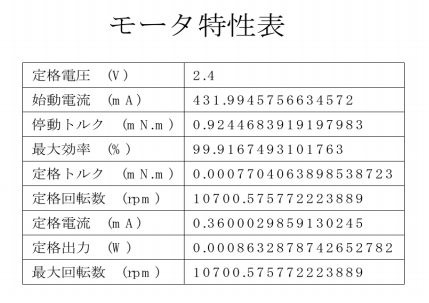
\includegraphics[width=7cm]{./Image/characteristicTable.png}
    }
    \caption{タイトルと特性表の画像}
	\label{fig:toku_gazou}
\end{figure}

\subsection{特性グラフ生成}\label{sub:toku_gurahu}
\ref{sub:csv_scan}節、\ref{sub:youso_kiso}節で求めた要素の配列を用いて、特性グラフを生成する。
処理の流れを以下に示す。
\begin{enumerate}
    % \item 配列torqueに、torque\_defaultを格納する
    % \item 配列currentに、current\_defaultを格納する
    % \item 配列speedに、angularvelocity\_defaultから\ref{siki:speed}式を適用した値を格納する
    % \item current\_defaultが0か判定し、以下の処理を行う
    % \begin{enumerate}
    %     \item 0だった場合、配列efficiencyに、0を格納する
    %     \item 0ではない場合、以下の処理を行う
    %     \begin{enumerate}
    %         \item current\_defaultと、voltage\_defaultを用いて\ref{siki:in}式から、0.0秒段階の入力の値を保持するinput\_defaultに代入する
    %         \item torque\_defaultと、angularvelocity\_defaultを用いて\ref{siki:out}式から、0.0秒段階の出力の値を保持するoutput\_defaultに代入する
    %         \item 配列efficiencyに、input\_defaultと、output\_defaultを\ref{siki:effi}式に適用した値を格納する
    %     \end{enumerate}
    % \item 配列outputに、torque\_defaultと、angularvelocity\_defaultを\ref{siki:out}式に適用した値を格納する
    % \end{enumerate}
    \item x軸に配列torqueを、y軸に配列currentを指定し、ライブラリmatplotlib(表\ref{tab:libr}参照)を用いてグラフを生成し、画像として保存する
    \item 1.の処理に対して、y軸に配列speedを指定した場合、y軸に配列efficiencyを指定した場合、y軸に配列outputを指定した場合を適用し、それぞれグラフを画像として保存する
\end{enumerate}
上記の処理で生成した4つのグラフを、それぞれ図\ref{fig:current}、図\ref{fig:speed}、図\ref{fig:effi}、図\ref{fig:output}に示す。

\begin{figure}[t]
    \begin{tabular}{cc}
        \begin{minipage}{0.45\hsize}
            \centering
            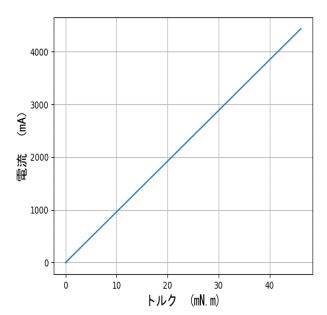
\includegraphics[width=.8\columnwidth]{./Image/current.png}
            \caption{「トルク $\times$ 電流」グラフ}
            \label{fig:current}
        \end{minipage}
        \hfill
        \begin{minipage}{0.45\hsize}
            \centering
            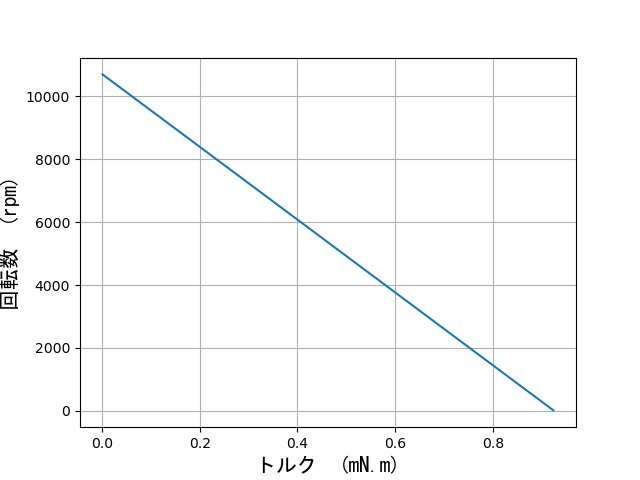
\includegraphics[width=.82\columnwidth]{./Image/speed.png}
            \caption{「トルク $\times$ 回転数」グラフ}
            \label{fig:speed}
        \end{minipage}\\\\
        \begin{minipage}{0.45\hsize}
            \centering
            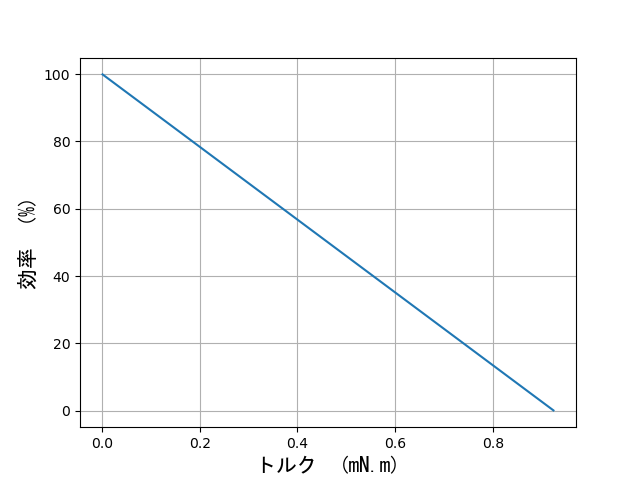
\includegraphics[width=.84\columnwidth]{./Image/efficiency.png}
            \caption{「トルク $\times$ 効率」グラフ}
            \label{fig:effi}
        \end{minipage}
        \hfill
        \begin{minipage}{0.45\hsize}
            \centering
            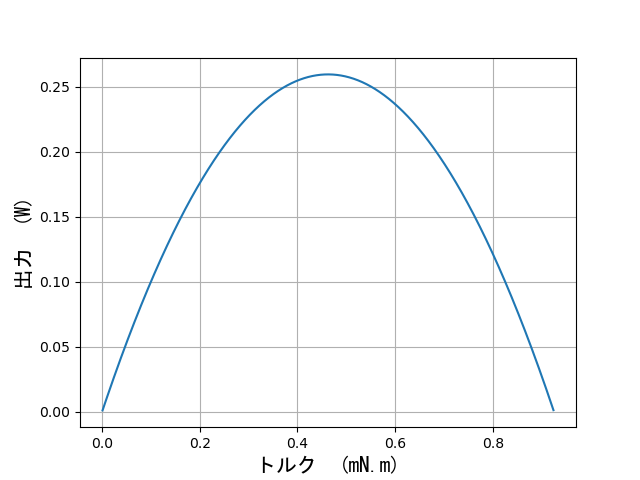
\includegraphics[width=.8\columnwidth]{./Image/output.png}
            \caption{「トルク $\times$ 出力」グラフ}
            \label{fig:output}
        \end{minipage}
    \end{tabular}
\end{figure}
% \begin{figure}[t]
% 	\centering
% 	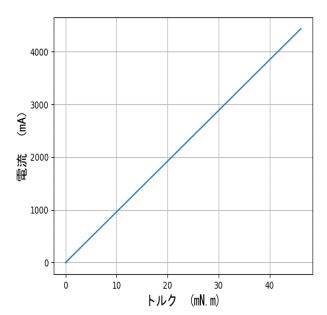
\includegraphics[width=7cm]{./Image/current.png}
% 	\caption{「トルク $\times$ 電流」グラフ}
% 	\label{fig:current}
% \end{figure}
% \begin{figure}[t]
% 	\centering
% 	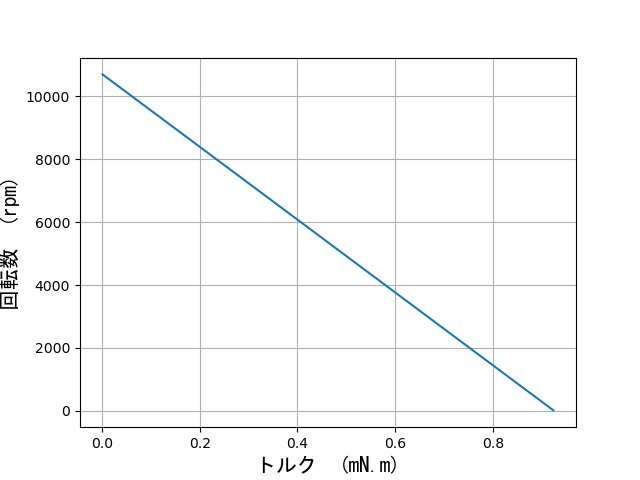
\includegraphics[width=7cm]{./Image/speed.png}
% 	\caption{「トルク $\times$ 回転数」グラフ}
% 	\label{fig:speed}
% \end{figure}
% \begin{figure}[t]
% 	\centering
% 	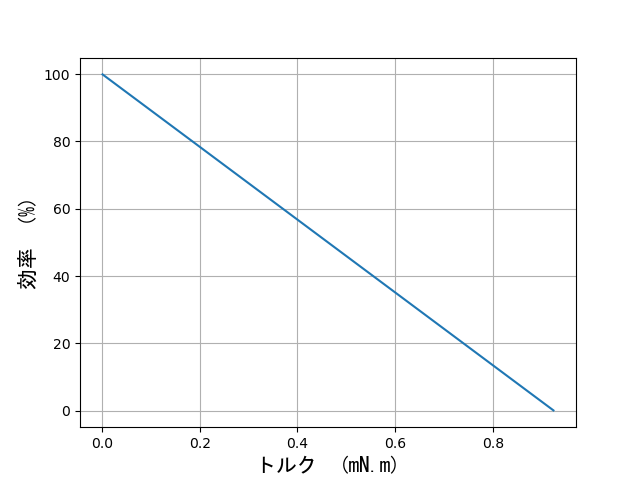
\includegraphics[width=7cm]{./Image/efficiency.png}
% 	\caption{「トルク $\times$ 効率」グラフ}
% 	\label{fig:effi}
% \end{figure}
% \begin{figure}[t]
% 	\centering
% 	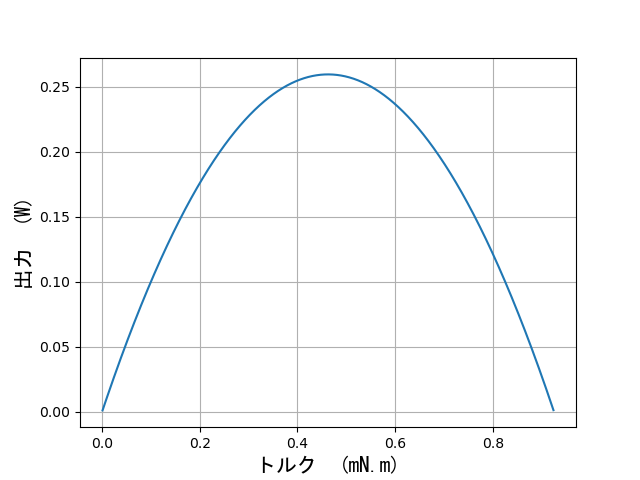
\includegraphics[width=7cm]{./Image/output.png}
% 	\caption{「トルク $\times$ 出力」グラフ}
% 	\label{fig:output}
% \end{figure}
\subsection{モータ特性表生成}\label{sub:}
\ref{sub:mortortoku}節と、\ref{sub:toku_gurahu}節で生成した合計5つの画像を、ライブラリreportlab(表\ref{tab:libr}参照)を用いて、PDFファイルに書き込み、モータ特性表を生成する。
モータ特性表のPDFファイルのファイル名は、「characteristicTable.pdf」で生成する。同じファイル名のPDFファイルがある場合、上書き保存する。
この処理で生成するモータ特性表を、図\ref{fig:tokuseihyou}に示す。
% \begin{figure}[t]
% 	\centering
% 	\fbox{
% 	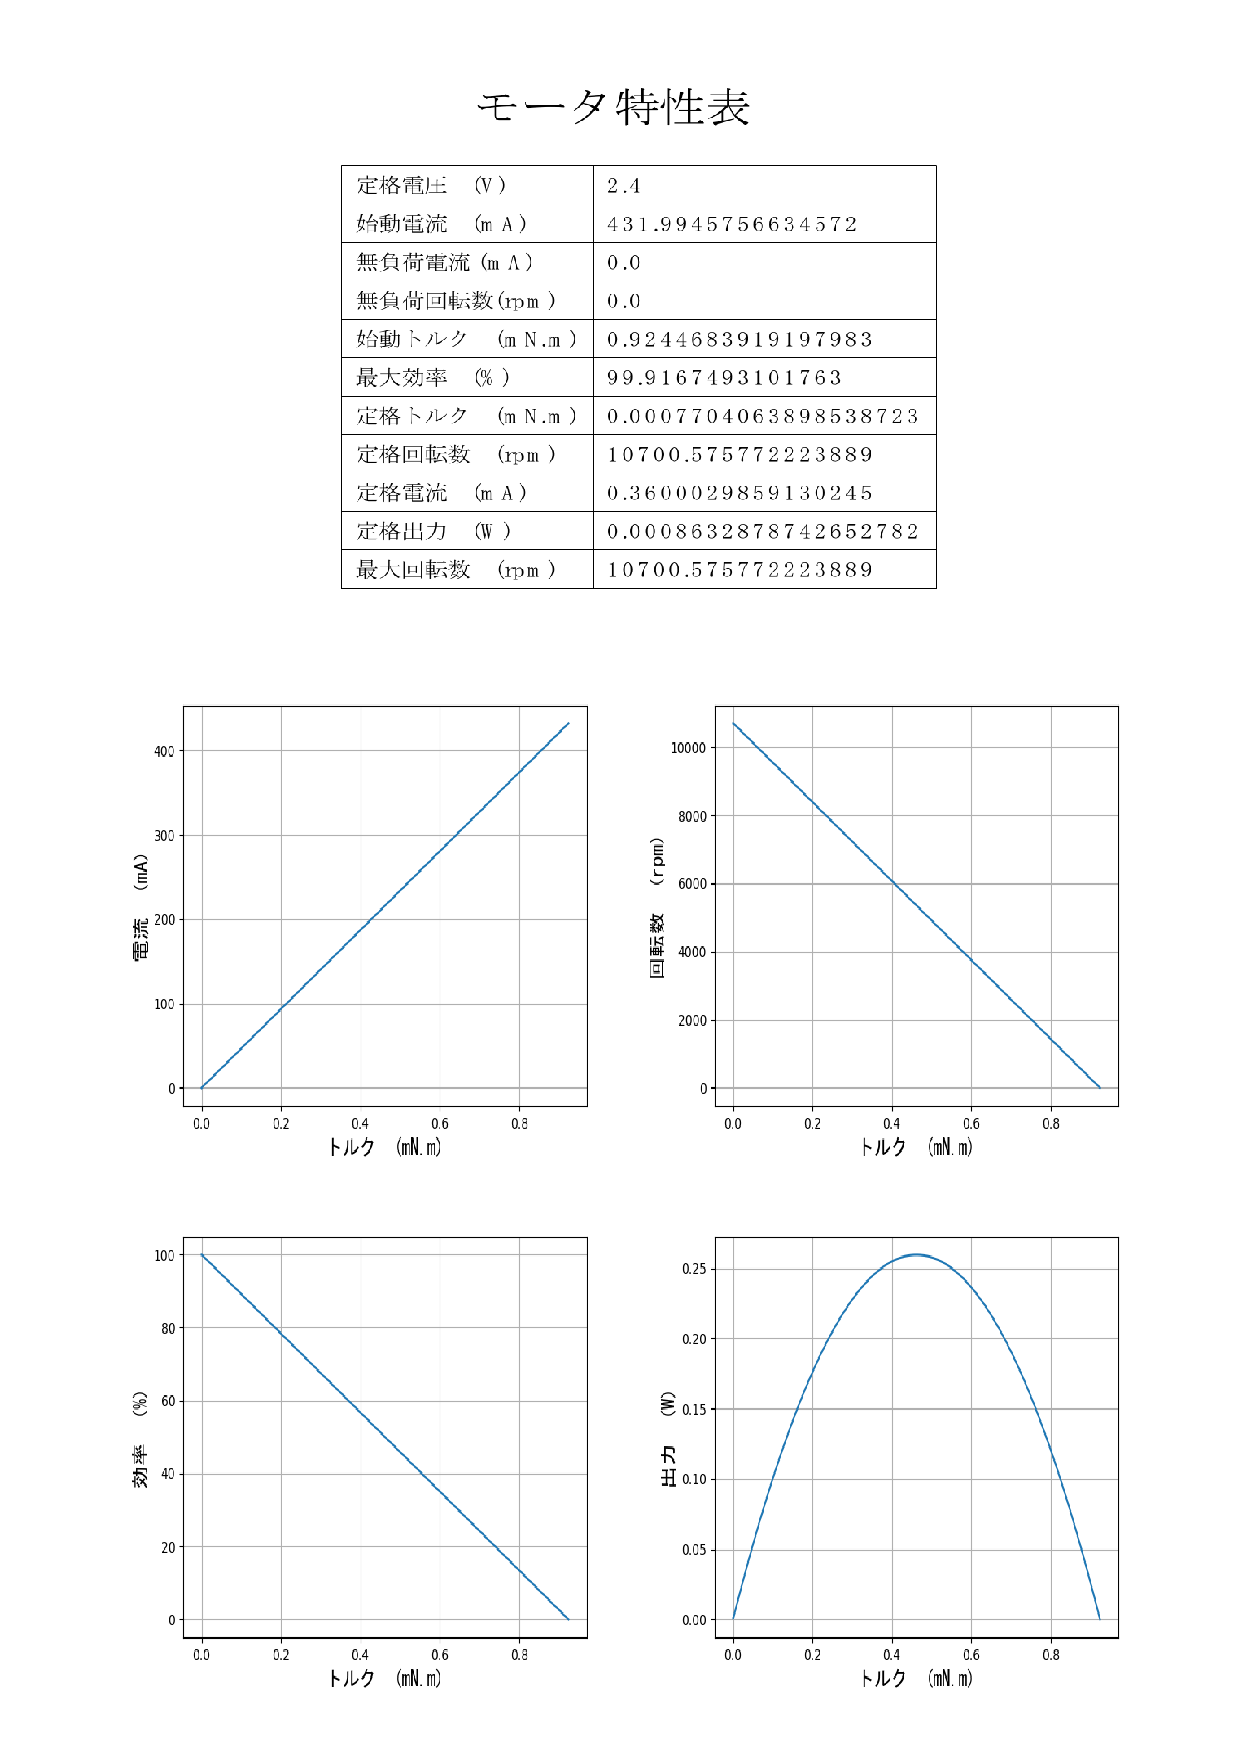
\includegraphics[width=16cm,pagebox=cropbox]{Image/characteristicTable.pdf} 
% 	}
% 	\caption{モータ特性表}
% 	\label{fig:tokuseihyou}
% \end{figure}